Detta kapitel innehåller en beskrivning av systemet utifrån ett tekniskt perspektiv. Inledningsvis redogörs för de tekniska förutsättningarna för systemet och ett antal tekniska termer förklaras. Sedan följer en detaljerad beskrivning av kommunikationsnätverket och de olika delsystemen: centralenheten, rörelselarmsenheten,  dörrlarmsenheten och störenheten.

\subsection{Teknisk bakgrund}

Ett vanligt larmsystem består av en centralstation där inställningar,
larmstatus och återställning av larmet hanteras samt ett antal periferienheter,
exempelvis dörrlarm, fönsterlarm och rörelselarm.
Periferienheterna skickar kontinuerligt information över ett nätverk till centralstationen som i sin tur tolkar informationen.

Nedan förklaras ett antal termer som är nödvändiga att känna till för fortsatt läsning av den tekniska beskrivningen av projektet.

\begin{description}

\item [Dörrlarm] Dörrlarm består vanligtvis av en sensor och en magnet som håller kontakten för att larmet inte ska aktiveras. Dessa har kontakt hela tiden när dörren är stängd, men så snart sensorn tappar kontakt med magneten, till exempel om dörren öppnas, skickas en signal till centralstationen och larmet aktiveras.
\item [Fönsterlarm] Fönsterlarm består av vibrationssensorer. Om vibrationerna för sensorn når över en bestämd nivå, till exempel om ett fönster krossas, skickar vibrationssensorn signaler till centralenheten som aktiverar ett larm.
\item [Rörelsedetektor] Rörelsedetektorer använder sig av ultraljud. Tiden det vid en viss tidpunkt tar för ljudvågorna att studsa tillbaka till sensorn beräknas. Denna tid jämförs med tiden det tagit för ljudvågorna att vid en tidigare tidpunkt studsa tillbaka till sensorn. Rörelsedetektorn kan då bedömma om något har rört sig inom dess övervakningsområde.
\item [MD407] En laborationsdator som bygger på mikroprocessorn STM32F407, framtagen i ett examensarbete på Chalmers Tekniska Högskola av Fredrik Östman\cite{MD407}.
\item [CAN-kommunikation] För att enheter ska kunna kommunicera med varandra måste det finnas ett kommunikationsprotokoll och ett datanätverk. Controller Area Network (CAN) är ett sådant nätverk. Varje CAN-meddelande har ett elva bitars ID-fält och ett 64-bitars datafält.
\item [USART] Hårdvara som används för att överföra data mellan två enheter.
\end{description}
\smallskip
All kod är skriven i C eller assembler. För att underlätta arbetet används biblioteket STM32 F4.

\subsection{Systemöversikt}

Systemet består av ett antal enheter (MD407-kort) som ansluts till ett gemensamt CAN-nätverk, se figur 2. En centralenhet ansluts via USART till en PC där användaren kan ändra systemets inställningar samt läsa av information om systemet (olika typer av larm). Ett valbart antal periferienheter, med sensorer av olika slag, sköter övervakandet av intressanta lägen, så som fönster och dörrar, och skickar larmsignal till centralenheten vid misstänksam aktivitet.

I figur 3 förklaras mjukvaran i form av ett flödesdiagram.

\begin{figure}[ht]
	\centering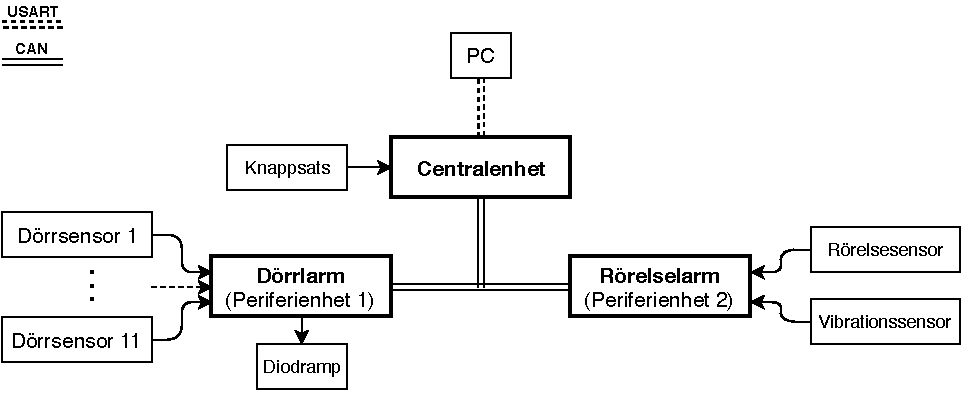
\includegraphics[width=0.8\textwidth]{figurer/systemoversiktfigur1.pdf}
	\caption{Översikt av hur larmsystemet är sammansatt.}
	\label{figur:översikt}
\end{figure}

\begin{figure}[h!]
	\centering\includegraphics[width=1\textwidth]{figurer/systemflode.pdf}
	\caption{Flödesschema för samtliga enheter samt deras kommunikation till varandra och uppkopplad PC.}
	\label{figur:flöde}
\end{figure}

\newpage
\subsection{Funktionella systemkrav}

Systemet har ett antal krav från kunden. Dessa är sammanställda i tabell \ref{tabell:krav}.

\begin{table}[h!]
\caption{Krav på grundsystemet utifrån kundens beskrivning. P1 står för periferienhet 1 (dörrlarm), P2 för periferienhet 2 (rörelselarm), S för störenhet, C för centralenhet och N för nätverk.}
\label{tabell:krav}
\centering
\begin{tabular}{| l | l | p{0.8\linewidth}|}
\hline
\textbf{ID} & \textbf{Komponent} & \textbf{Beskrivning} \\ \hline
K01 & P1 & Om en dörr stått öppen en viss tid ska enheten larma lokalt. Efter ytterligare en tid ska enheten larma centralenheten. \\ \hline
K02 & C & När larmet gått ska det fortsätta tills en fyrsiffrig kod matas in på knappsatsen vid centralenheten. \\ \hline
K03 & P1 & Flera dörrar ska kunna larmas med samma enhet. \\ \hline
K04 & N & Nätverket ska ha stöd för flera dörrlarmsenheter samtidigt. \\ \hline
K05 & P1 & Antalet dörrar för en dörrenhet ska kunna konfigureras när enheten startas genom  USART,  via  CAN  från  centralenheten  eller genom strömbrytare. \\ \hline
K06 & P1 & Larmet för enskilda dörrar ska kunna inaktiveras och aktiveras genom att på centralenheten ange en fyrsiffrig kod och ett ID för dörren. Om en dörr är olarmad ska en grön lysdiod lysa. Via centralenheten ska man kunna konfigurera hur länge varje dörr tillåts vara öppen innan larmet går. \\ \hline
K07 & P2 & Enheten ska använda en ultraljudsbaserad avståndsmätare som rörelselarm. Enheten ska larma centralenheten om någon eller något rör sig inom dess räckvidd. \\ \hline
K08 & P2 och C & Från  centralenheten  ska  man  kunna  justera  känsligheten  för avståndsmätaren på periferienhet 2, samt kalibrera den. \\ \hline
K09 & P2 & Enheten ska använda en vibrationssensor, som kan monteras på en fönsterruta, som rörelselarm. Enheten ska larma centralenheten om fönsterrutan krossas. \\ \hline
K10 & S & Störenheten ska skicka stora volymer data på CAN-bussen. Volymen data som skickas ska kunna justeras. \\ \hline
K11 & C & När ett larm uppstår ska centralenheten kommunicera det till en ansluten PC via  USART. \\ \hline
K12 & C & När  systemet  startas  ska  centralenheten  kunna  konfigureras  via  USART  så  att  den känner till vilka enheter som finns anslutna och hur de är konfigurerade. \\ \hline
K13 & C & Centralenheten ska larma om någon periferienhet går sönder eller kopplas från nätverket. \\ \hline
\end{tabular}
\end{table}


\subsection{Delsystem}
Här förklaras mer djupgående vad varje delsystem gör och hur de fungerar.
\subsubsection{Kommunikationsnätverk}

CAN används för kommunikation mellan centralenheten och periferienheterna. Dessa enheter kopplas samman med en RJ11-kabel som ansluts till första CAN-porten (CAN1-port) på respektive MD407-kort. Pinnar PB8 och PB9 på MD407-korten används som in- respektive utdata-pin för CAN.

CAN-system kan, till skillnad från master/slave-system, sända och mottaga meddelanden till flera noder simultant. För att undvika busskollission och försäkra att bussen används av endast en användare åt gången prioriterar CAN meddelanden med lägre ID-nummer. 

ID-fältets elva bitar delas upp på meddelandetyp, riktning till eller från centralenheten, samt enhets-ID (se tabell \ref{systemöversikt_can:1}). Systemet stödjer upp till och med 32 olika enheter med ID:n som ligger mellan 0x0 och 0x1F.


\begin{table}[h!]
\caption{Bitfördelning i ett CAN-meddelande ID-fält}
\label{systemöversikt_can:1}
\centering
\begin{tabular}{|l|l|l|l|l|l| }
\hline
\textbf{Bitnummer} & 11 & 10 & 9 - 6 & 5 - 1 \\
\hline
\textbf{Funktion} & Prioritet & Till/från centralenhet & Meddelandetyp & Enhets-ID \\
\hline
\textbf{Möjliga värden} & 0: Hög prioritet & 0: Till centralenheten & 0x0 - 0xF & 0x0 - 0x1F \\
\textbf{} & 1: Låg prioritet & 1: Från centralenheten & & \\
\hline
\end{tabular}
\end{table}

Prioriteringssystemet baseras på meddelandetypen i ID-fältet, vilket garanterar att viktiga meddelanden prioriteras och överförs före andra i bussen oavsett enhets-ID. Dataöverföring på CAN-bussen blir således mer effektivt och minskar eventuell förlust i överföring av viktiga meddelanden.

Ett CAN-meddelande kan innehålla som högst åtta bytes data. All data som skickas via CAN och även meddelandetyp i ID-fältet krypteras på grund av säkerhetsskäl.

Eftersom meddelanden i ett CAN-system skickas från en nod till alla andra noder, utan hänsyn till meddelandets mottagare, införs ett meddelandefilter på varje nod. Periferienheternas meddelandefilter konfigureras så att enbart meddelanden från centralenheten tas emot. Centralenheten tar emot alla meddelanden med riktning till centralenheten. På detta sätt undviker systemet onödiga anrop av CAN-avbrott och det sparas på resurser.

\subsubsection*{De olika typerna av meddelanden}

Systemet har stöd för 16 olika meddelandetyper. De olika meddelandetyperna som används är alarm (ALARM), bekräftelse (ACK), kommando (CMND), konfiguration (CONF) och ping (REQST), se tabell 3.

\begin{table}[h!]
\caption{Meddelandetyper och deras motsvarande ID:n}
\label{systemöversikt_can:2}
\centering
\begin{tabular}{|l|l| }
\hline
\textbf{Meddelandetyp} & \textbf{ID} \\
\hline
ALARM & 0x0 \\
\hline
ACK & 0x1 \\
\hline
CMND & 0x2\\
\hline
CONF & 0x3 \\
\hline
REQST & 0x4 \\
\hline
\end{tabular}
\end{table}

\begin{description}
    \item [Alarm] Ett alarm-meddelande skickas från en periferienhet till centralenheten när ett larm uppstår. Centralenheten skickar i sin tur ett alarm-meddelande till en viss periferienhet när ett larm avaktiverats av användaren.
    \item [Bekräftelse] När en enhet mottager ett meddelande skickar den en bekräftelse till enheten som skickade meddelandet.
    \item [Kommando] Ett kommando-meddelande skickas från centralenheten till en viss periferienhet när ett kommando skrivs in i terminalfönstret på användarens PC, exempelvis kalibrering av avståndsmätaren.
    \item [Konfiguration] Ett konfigurationsmeddelande skickas, liksom kommando-med-delanden, från centralenhten när användaren skriver in ett kommando i PC:ns terminalfönster. Exempel på dessa meddelanden är att ändra rörelsemätarens känslighet eller konfigurera hur många dörrar en dörrlarmsenhet ska ha stöd för.
    \item [Ping] Centralenheten skickar ett anrop var femte sekund till samtliga enheter på nätverket. Enheterna förväntas besvara anropet genom att skicka ett anrop-meddelande tillbaka.
\end{description}
	
\subsubsection{Centralenheten}

Centralenheten är ansvarig för att hålla information om de olika enheterna på nätverket, kommunicera med de, samt larma via den anslutna PC:n när ett larm utlöses.

Larm avaktiveras med hjälp av knappsatsen. För att avgöra om en knapp på knappsatsen trycks ner används \textit{pollning}. Metoden innebär att mjukvaran undersöker aktuell status på knappsatsen och returnerar motsvarande nedtryckta tangents värde. Om ingen tangent är nedtryckt returneras ett värde som representerar detta.
Mjukvaran läser på detta vis av knappsatsen och lägger in nedtryckningarna (siffrorna) i en buffert.
Programmet läser av bufferten när användaren trycker på D-knappen - likt Enter-knappens funktion på ett vanligt tangentbord - och jämför denna med alla pin-koder för samtliga periferienheters sensorer.
Om bufferten matchar en pin-kod vars sensor har flaggat för larm, skickar centralenheten ett CAN-meddelande till den enhet som sensorn sitter på.

Centralenheten skickar ett kommando- eller konfigurationsmeddelande om den aktuella inmatningen på USART, som även den lägger sig i en buffert, matchar ett kommandos namn
från kommandolistan (se tabell 4), vilken finns i centralenhetens mjukvara. Ett kommando har ett namn och ett CAN-meddelande. Om kommandots CAN-meddelande är av typen \textit{configuration}, ber centralenheten
användaren att skriva in ett nytt värde för konfigurationen. Centralenheten ber även användaren att skriva in vilken enhet meddelandet ska skickas till.

\begin{table}[h]
\caption{Lista över kommandon som användaren kan skriva in i USART.}
\scalebox{0.95}{\hskip-1.5cm
\begin{tabular}{|l|l|l|l|}
\hline
\textbf{Kommando} & \textbf{Beskrivning} & \textbf{Typ av meddelande} \\ \hline
calib & Kalibrerar ultraljudsmätaren på rörelseenheten & Command \\ \hline
config & Konfigurerar enheten och sensorn som angivs efter kommandot & Configuration \\ \hline
deact & Inaktiverar sensor som specificeras efter kommandot & Configuration \\ \hline
\end{tabular}}
\end{table}

\subsubsection{Periferienhet 1: Dörrlarm}

Periferienhet 1 är ett dörrlarm. Enheten kopplas till dörrsensorer och hanterar dörrarna enligt separata inställningar för varje dörr. Dörrlarmet kan konfigureras och styras genom centralenheten.

\subsubsection*{Dörrsensorn}

Dörrsensorn består av en magnetisk sensor med två ledare som kopplas till enheten, samt en tillhörande magnet (se figur 4). När sensorn är tillräckligt nära magneten sluts kretsen. Sensorn monteras på dörrkarmen och magneten på dörren, på så sätt att sensorn är tillräckligt nära magneten när dörren är stängd för att kretsen ska slutas. Då dörren öppnas bryts kretsen.

\begin{figure}[h!]
	\centering\includegraphics{figurer/dorrsensor.pdf}
	\caption{Kopplingsschema för dörrsensorn.}
	\label{figur:dörrsensor}
\end{figure}

Dörrsensorerna är kopplade till logiknivå hög (1) på ena ledaren och en allmän användnings-pin (GPIO-pin) på den andra. När dörren är stängd och kretsen är sluten läses ett logiskt högt värde på pinnen. GPIO-pinnen är konfigurerad som ingång av typen \textit{pull-down}, så när kretsen är bruten sätts ingången till låg (0).

Varje dörrsensor-pin är kopplad till en extern avbrottslina (EXTI) som är konfigurerad att generera avbrott på fallande och stigande flank, alltså både då dörren öppnas och då den stängs. Samma avbrottshanterare används för alla dörrsensor-avbrott, och avbrottshanteraren läser av samtliga dörrsensorer för att sätta respektive status på dörrarna.

Då samma avbrottshanterare används för alla dörrsensorer, används avbrottslinorna 5-9 och 10-15 där fem respektive sex avbrottslinor är kopplade till samma avbrottshanterare. Nio av dessa pinnar används för dörrsensorer.

Enhetens huvudprogram hanterar de olika larmfunktionerna beroende på dörrarnas och timernas status.

\subsubsection*{Dörrsystemet}

Varje dörrsensor har ett unikt dörr-ID och behandlas separat i periferienheten som en dörr. Dörrarna har inställningar för om larmet ska vara aktivt eller inaktivt, samt en timer för hur länge en dörr med larmstatus aktiv ska få vara öppen innan ett larm skickas till centralenheten. Varje dörr har tre statusar: en status för dörrens status (öppen/stängd) och två larmstatusar, en lokal larmstatus som sätts som aktiv då dörren öppnats och avbrottet för dörren genererats, och en central larmstatus som sätts som aktiv då timern har räknat ned och larm skickats till centralenheten.

\subsubsection{Periferienhet 2: Rörelselarm}

Periferienhet 2 är ett rörelselarm bestående av en vibrationssensor som kan fästas på exempelvis ett fönster och en ultraljudsmätare som mäter om något rört sig inom dess övervakningsområde.

\subsubsection*{Vibrationssensorn}

Vibrationssensorn använder SW-18010P för att mäta vibrationer. Känsligheten kan justeras med en potentiometer, ett reglerbart motstånd, på vibrationssensorn.

\begin{figure}[h!]
	\centering\includegraphics{figurer/vibsensor.pdf}
	\caption{Kopplingsschema för vibrationssensorn.}
	\label{figur:vibsensor}
\end{figure}

Vibrationssensorn har fyra pinnar - VCC, GND, D0 och A0 - varav de tre första kopplas till en MD407-enhet (se figur 5). När vibrationssensorn triggas blir D0-pinnen logiskt låg (0).

D0 är ansluten till PD0 på MD407, som är konfigurerad att generera avbrott på negativ flank. När vibrationssensorn triggas genereras ett avbrott och en flagga sätts.
Flaggans värde undersöks i programmets huvudloop. Om värdet är logiskt högt (1) skickar periferienheten ett CAN-meddelande till centralenheten, förutsatt att ett meddelande inte redan har skickats.
När centralenheten larmar av mottager periferienheten ett meddelande och nollställer larmet för vibrationssensorn.


\subsubsection*{Ultraljudsmätaren}

Ultraljudsmätaren skickar ut ultraljud, med en vinkel på 15 grader, fyra gånger per sekund. Tiden mäts genom att använda SysTick, vilken räknar i mikrosekunder.
Sensorn larmar då något rört sig mer än ett visst gränsvärde (i centimeter) sedan förra mätningen. Detta gränsvärde är justerbart från centralenheten, genom ett kommando i terminalfönstret på ansluten PC.

Ultraljudsmätaren har fyra pinnar - VCC, GND, Trig och Echo - varav alla kopplas till en MD407-enhet (se figur 6).
Trig-pinnen är ansluten till PD1, som är konfigurerad som utport.
Echo-pinnen är ansluten till PD2, som är konfigurerad som inport.
För att mätaren ska skicka ut ultraljud sätter mjukvaran Trig-pinnen till logiskt hög (1) i 10 mikrosekunder och återställer sedan pinnen till logiskt låg (0).

\begin{figure}[h!]
	\centering\includegraphics{figurer/ultrasensor.pdf}
	\caption{Kopplingsschema för ultraljudsmätaren.}
	\label{figur:ultrasensor}
\end{figure}

En mätning går till på sådant vis att mjukvaran aktiverar mätaren samtidigt som den sätter en tidsstämpel. Sedan tar den en ny tidsstämpel då ultraljudet återvänder till mätaren genom eko (echo-pinnen blir logiskt hög (1)).
Periferienheten jämför sedan tidsstämplarna och avgör om något rört sig mer än vad gränsvärdet tillåter.
Om den uppmätta distansen överskrider gränsvärdet genereras ett mjukvaruavbrott i periferienheten, vilket sätter en flagga och ett larm skickas till centralenheten. Periferienheten nollställer larmet för ultraljudsmätaren på samma vis som för vibrationssensorn.

\subsubsection{Störenheten}

För att undersöka nätverksbeteende vid olika belastningsgrader byggs en störenhet som simulerar en defekt periferienhet eller en ovälkommen anfallare som skickar stora volymer data på CAN-bussen. Störenheten är uppbyggd med samma princip som en DoS-attack, vilket förhindrar kommunikationen mellan centralenheten och periferienheterna. När störenheten startas ligger den och väntar på att spela in ett meddelande mellan enheterna. När ett meddelande spelats in förfalskar störenheten meddelandets ID. Genast efter det skickas ett förbestämt antal meddelanden som innehåller 8 bytes data med det förfalskade ID:t på CAN-bussen, denna typ av attack är känd som en återspelnings-attack. 

CAN-kommunikationssystem konfigureras för att kunna överföra upp till 750 Kbps, vilket är mer än den totala datamängden som störenheten kan skicka per sekund. Mottagaren kan däremot inte hantera mottagna meddelanden lika snabbt som störenheten skickar meddelandena. CAN-kontrollern har tre först-in-först-ut inkorgar som kan ta emot som högst tre meddelanden vid samma tillfälle. Störenheten utnyttjar detta för att blockera någon enhet genom att tvinga enheten att hantera ett stort antal av förfalskade meddelanden. Riktiga meddelanden skickas fortfarande över CAN-bussen men tas inte emot av mottagaren på grund av dess otillgänglighet.

Förutom meddelandesmottagning förhindrar störenheten även användarens aktivitet, eftersom CAN-avbrott genereras ständigt och dessa kräver hantering.

Hur en enhet klarar av olika belastningsgrader av mottagna meddelanden kan undersökas, då det finns möjlighet att konfigurera antal meddelanden och datamängd som skickas från störenheten.



